% !TeX root = ../main.tex


\section{Experiments}
\label{sec:exp}
\subsection{Experimental Setup}
\label{sec:exp_setup}
\noindent{\textbf{Datasets.}}
We use four Amazon domains~\cite{amazon} (Toys, Beauty, Clothing, Sports) and MovieLens~\cite{ml-1m} to test generalization across domains and platforms on the Web, with 5-core filtering and leave-one-out splits.
Preprocessing and statistics are in App.~\ref{app:datasets} (Tab.~\ref{tab:dataset_stats}).

% \vspace{+0.1cm}
% \noindent{\textbf{Baselines.}}
% Besides the ID-based SASRec~\cite{sasrec}, the baselines form two groups, as in Tab.~\ref{tab:perf_task2} (details in Appendix~\ref{app:exp_details}).
% 1) \textbf{Text-based models}: BERT~\cite{bert}, a small text encoder; SLIM and SLIM$^{+}$~\cite{slim}, which embed items with BERT and its CF-trained student LLM, respectively; LLMEmb~\cite{llmemb} and LLM2Rec~\cite{llm2rec}, which inject CF into LLM embeddings; and $\text{LLM}_{\text{Vanilla}}$ and $\text{LLM}_{\text{SFT}}$, an untuned LLM and one tuned with standard SFT (Eq.~\ref{eq:sft_loss}).
% 2) \textbf{Multimodal-based models}: CLIP~\cite{clip}, a small image--text encoder; $\text{VLM}_{\text{Prompt}}$~\cite{vlm_prompt}, NoteLLM-2~\cite{notellm2}, and I-LLMRec~\cite{illmrec}, which build multimodal item embeddings via zero-shot prompting, item-level fusion, and CLIP features fed to an LLM, respectively; MLLM-MSR~\cite{mllmmsr}, which summarizes item images and user preferences into text with a VLM; and $\text{VLM}_{\text{Vanilla}}$ and $\text{VLM}_{\text{SFT}}$, the VLM counterparts of the LLM variants.

\vspace{+0.1cm}
\noindent{\textbf{Baselines.}}
The baselines form three groups (details in App.~\ref{app:exp_details}).
\begin{itemize}[wide=0pt]
    \item \textbf{ID-based models}: GRU4Rec~\cite{gru4rec}, FMLP~\cite{fmlp}, DiffuRec~\cite{diffurec}, and SASRec~\cite{sasrec}, which learn item embeddings from interactions alone.
    \item \textbf{Text-based models}: BERT~\cite{bert}, a small text encoder; SLIM and SLIM$^{+}$~\cite{slim}, which embed items with BERT and its CF-trained student LLM, respectively; LLMEmb~\cite{llmemb} and LLM2Rec~\cite{llm2rec}, which inject sequence-level CF into LLM embeddings; and $\text{LLM}_{\text{Vanilla}}$ and $\text{LLM}_{\text{SFT}}$, an untuned LLM and one tuned with standard SFT (Eq.~\ref{eq:sft_loss}).
    \item \textbf{Multimodal-based models}: CLIP~\cite{clip}, a small image--text encoder; $\text{VLM}_{\text{Prompt}}$~\cite{vlm_prompt}, NoteLLM-2~\cite{notellm2}, and I-LLMRec~\cite{illmrec}, which embed items via zero-shot prompting, item-level fusion, and CLIP features fed to an LLM, respectively; MLLM-MSR~\cite{mllmmsr}, which summarizes item images and user preferences into text with a VLM; and $\text{VLM}_{\text{Vanilla}}$ and $\text{VLM}_{\text{SFT}}$, the VLM counterparts of the LLM variants.
\end{itemize}

\vspace{+0.1cm}
\noindent{\textbf{Evaluation Protocol.}} 
We use full-ranking evaluation~\cite{negative_sampling} in two settings.
In the VLM2Rec setting, each method encodes the user's history and ranks all items by $\text{s}(\mathbf{e}_u,\mathbf{e}_i)$.
In the $\text{VLM2Rec}_{\text{plug}}$ setting, a linear adapter (or a baseline's own adapter, when specified) maps each method's frozen item embeddings to the hidden size ($d{=}128$) of SASRec~\cite{sasrec}; only the adapter and the backbone are trained, so all methods share the same inference cost.
We also evaluate DiffuRec~\cite{diffurec}, FMLP~\cite{fmlp}, and GRU4Rec~\cite{gru4rec} as SR backbones (Tab.~\ref{tab:add_backbones}).
We report H@$K$ and N@$K$ ($K \in \{10,20\}$) averaged over five seeds; all gains pass a paired $t$-test ($p<0.05$).


\vspace{+0.1cm}
\noindent{\textbf{Implementation Details.}} We build VLM2Rec and the VLM-based baselines on Qwen2.5-VL-3B and the LLM-based baselines on Qwen2.5-3B, where applicable; tuned variants use LoRA~\cite{lora}.
$\mathcal{N}_u$ and $\mathcal{C}$ are built from in-batch items, and Tab.~\ref{tab:negative_sampling} tests hard negatives for $\mathcal{N}_u$.
Other training details are in App.~\ref{app:implementation_details}.

\subsection{Main Results}
\label{sec:exp_main}
% VLM2Rec outperforms all baselines with statistical significance, and $\text{VLM2Rec}_{\text{plug}}$ also performs best in its setting (Tab.~\ref{tab:perf_task2}).
% Three observations from the baseline groups explain these gains.
VLM2Rec and $\text{VLM2Rec}_{\text{plug}}$ significantly outperform all baselines (Tab.~\ref{tab:perf_task2}), as three observations explain.

\begin{itemize}[wide=0pt]
    \item \textbf{O1: Semantics alone cannot replace sequence-level CF.}
    SFT improves both Vanilla models by 17--57\% in N@20 across the two settings, and SLIM stays near BERT, whereas $\text{SLIM}^{+}$, which embeds with its CF-trained LLM, improves sharply.
    VLM2Rec keeps the CF that SFT injects, as $\mathcal{L}_{\text{WPCL}}$ retains the SFT objective and only reweights its negative term.
    The encoder needs CF even when the SR backbone learns CF on its own: in the $\text{VLM2Rec}_{\text{plug}}$ setting, encoders trained without CF (BERT, CLIP, $\text{VLM}_{\text{Prompt}}$, and the Vanilla models) all trail even the ID-based SASRec.
    \item \textbf{O2: Correcting the collapse turns vision into consistent gains.}
    Images complement titles: $\text{VLM}_{\text{Vanilla}}$ outperforms $\text{LLM}_{\text{Vanilla}}$ in both settings, as does CLIP over BERT.
    Yet $\text{VLM}_{\text{SFT}}$, though better than $\text{LLM}_{\text{SFT}}$ on most metrics, trails it on several in both settings: SFT-amplified collapse leaves the visual modality under-optimized, causing negative transfer when fused.
    VLM2Rec, which differs from $\text{VLM}_{\text{SFT}}$ only in its objectives, outperforms all baselines, including the multimodal runners-up ($\text{VLM}_{\text{SFT}}$ or I-LLMRec), as does $\text{VLM2Rec}_{\text{plug}}$ in its setting.
    $\mathcal{L}_{\text{WPCL}}$ strengthens each user's weaker modality and $\mathcal{L}_{\text{CRTR}}$ aligns each user's similarity structures across the two modalities, so fusion adds visual evidence instead of causing negative transfer (Sec.~\ref{sec:modality_mute}).
    \item \textbf{O3: The item embeddings carry these gains into SR backbones.}
    Because the $\text{VLM2Rec}_{\text{plug}}$ setting passes only the frozen item embeddings to the backbone, the same trends there show that VLM2Rec's item embeddings themselves carry sequence-level CF (O1) and balanced multimodal semantics (O2).
    Accordingly, $\text{VLM2Rec}_{\text{plug}}$ also performs best with DiffuRec, FMLP, and GRU4Rec (Tab.~\ref{tab:add_backbones}), serving as plug-and-play item representations.
\end{itemize}


\begin{figure}[!t]
    \centering
    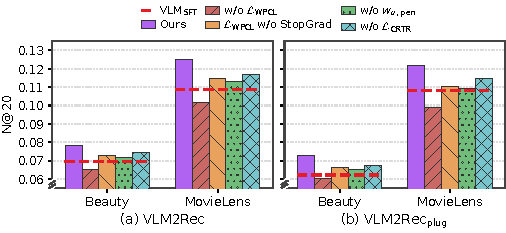
\includegraphics[width=\columnwidth]{figures/ablation.pdf}
    \vspace{-0.3cm}
    \caption{Ablation of (a) VLM2Rec and (b) $\text{VLM2Rec}_{\text{plug}}$.}
    \label{fig:ablation_cf}
    \Description{Two bar-chart panels, (a) VLM2Rec and (b) VLM2Rec-plug with SASRec, each with Beauty and MovieLens groups on a shared y-axis. The full model outperforms all four ablations in every group, with the largest decrease when WPCL is removed. Red dashed lines show the VLM SFT baseline.}
\end{figure}

% !TeX root = ../main.tex
\begin{table}[!t]
\centering
\caption{Generic gradient modulation vs. $\mathcal{L}_{\text{WPCL}}$ in the $\text{VLM2Rec}_{\text{plug}}$ setting (SASRec, N@20).}
\vspace{-0.2cm}
\label{tab:gradient_balancing}
% \footnotesize
\setlength{\tabcolsep}{5pt}
\renewcommand{\arraystretch}{0.7}
\begin{tabular}{@{}llcccc@{}}
\toprule
\textbf{Dataset} & \textbf{Method} & \textbf{\TEXTset} & \textbf{\VISIONset} & \textbf{\FUSIONset} & \textbf{Gap} (\%) \\
\midrule
\multirow{4}{*}{Beauty}
 & $\text{VLM}_{\text{SFT}}$   & 0.0650 & 0.0587 & 0.0622 & 10.7 \\
 & OGM-GE~\cite{modality_balancing_OGM-GE_1}    & 0.0677 & 0.0616 & 0.0632 & 9.9 \\
 & AGM~\cite{modality_balancing_AGM_2}       & 0.0664 & 0.0605 & 0.0648 & 9.8 \\
 & $\mathcal{L}_{\text{WPCL}}$ only & 0.0667 & 0.0638 & 0.0673 & 4.5 \\
\midrule
\multirow{4}{*}{MovieLens}
 & $\text{VLM}_{\text{SFT}}$   & 0.1100 & 0.0953 & 0.1082 & 15.4 \\
 & OGM-GE~\cite{modality_balancing_OGM-GE_1}    & 0.1087 & 0.0965 & 0.1068 & 12.6 \\
 & AGM~\cite{modality_balancing_AGM_2}       & 0.1120 & 0.1008 & 0.1108 & 11.1 \\
 & $\mathcal{L}_{\text{WPCL}}$ only & 0.1136 & 0.1108 & 0.1148 & 2.5 \\
\bottomrule
\end{tabular}
\end{table}


\subsection{Analysis of Mitigating Modality Collapse}
\label{sec:modality_mute}
VLM2Rec first rebalances optimization: it closes the text--vision gradient gap of $\text{VLM}_{\text{SFT}}$ and even tilts it slightly toward vision, since $\mathcal{L}_{\text{WPCL}}$ adds an extra gradient to each user's weak modality, mostly vision, and $\mathcal{L}_{\text{CRTR}}$ aligns each user's similarity distributions across the two modalities (Fig.~\ref{fig:drop_grad} right).
This restores the visual embedding geometry: visual separability now matches or exceeds that of text, and visual uniformity improves sharply (Tab.~\ref{tab:ali_uni_clo}).
Consequently, the \TEXTset{}--\VISIONset{} gap, which $\text{VLM}_{\text{SFT}}$ widened, nearly closes (1.3\% and 2.0\%), and fusion turns from negative transfer into synergy: \FUSIONset{} > \TEXTset{} and \FUSIONset{} > \VISIONset{} (Fig.~\ref{fig:drop_grad} left).
Across additional domains, model families, and scales, VLM2Rec consistently narrows the \TEXTset{}--\VISIONset{} gap and improves \FUSIONset{} (Fig.~\ref{fig:drop_grad_toys_clothing} and Tab.~\ref{tab:modality_collapse_backbones}).
Even an open-source embedding-pretrained VLM (Qwen3-VL-Embedding) shows a sizable \TEXTset{}--\VISIONset{} gap, which VLM2Rec narrows while improving \FUSIONset{} (Tab.~\ref{tab:qwen3_vl_embedding}).

% We revisit this aggregate pattern at the user level in Section~\ref{sec:user_stratification}.

% !TeX root = ../main.tex
\begin{table}[!t]

\centering
\caption{Modality embedding replacement experiments on state-of-the-art models. \protect\colorbox{bestcolor}{\textbf{Bold}}/\protect\colorbox{secondcolor}{\underline{underline}}: best/second best.}

\label{tab:modality_rec}
\resizebox{\linewidth}{!}{
    \renewcommand{\arraystretch}{0.7}
    \begin{tabular}{lcccc}
    \toprule
    \multirow{2}{*}{\textbf{Embedding}}
    & \multicolumn{2}{c}{\textbf{UniSRec}~\cite{modrec_unisrec}}
    & \multicolumn{2}{c}{\textbf{TedRec}~\cite{modrec_tedrec}} \\
    \cmidrule(lr){2-3} \cmidrule(lr){4-5}
    & Clothing & MovieLens & Clothing & MovieLens \\
    \midrule
    BERT                              & 0.0308               & 0.1086               & 0.0332               & 0.1167               \\
    $\text{LLM}_{\text{SFT}}$         & 0.0325               & 0.1119               & 0.0348               & 0.1180               \\
    $\text{VLM}_{\text{SFT}}$ (Text)  & \secondscore{0.0328} & 0.1124               & \secondscore{0.0355} & \secondscore{0.1189} \\
    I-LLMRec (Text)                   & 0.0318               & \secondscore{0.1128} & \secondscore{0.0355} & 0.1184               \\
    \textbf{$\text{VLM2Rec}_{\text{plug}}$ (Text)}        & \bestscore{0.0336}   & \bestscore{0.1137}   & \bestscore{0.0362}   & \bestscore{0.1208}   \\
    \midrule
    \multirow{2}{*}{\textbf{Embedding}}
    & \multicolumn{2}{c}{\textbf{M3SRec}~\cite{modrec_m3srec}}
    & \multicolumn{2}{c}{\textbf{HM4SR}~\cite{modrec_hm4sr}} \\
    \cmidrule(lr){2-3} \cmidrule(lr){4-5}
    & Clothing & MovieLens & Clothing & MovieLens \\
    \midrule
    CLIP                      & 0.0322               & 0.1134               & 0.0277               & 0.1219               \\
    $\text{VLM}_{\text{SFT}}$ & 0.0338               & 0.1158               & 0.0328               & \secondscore{0.1261} \\
    I-LLMRec                  & \secondscore{0.0347} & \secondscore{0.1165} & \secondscore{0.0345} & 0.1259               \\
    \textbf{$\text{VLM2Rec}_{\text{plug}}$}       & \bestscore{0.0352}   & \bestscore{0.1176}   & \bestscore{0.0396}   & \bestscore{0.1315}   \\
    \bottomrule
    \end{tabular}
    }

\end{table}

\subsection{Ablation Study}
We ablate each component in both settings to examine its contribution (Fig.~\ref{fig:ablation_cf}).
Every component contributes, with $\mathcal{L}_{\text{WPCL}}$ the most critical, and both settings show the same ordering of variants.
Without $\mathcal{L}_{\text{WPCL}}$, the model underperforms $\text{VLM}_{\text{SFT}}$, as it neither injects sequence-level CF nor improves weak-modality discrimination.
Removing $w_{u,\text{pen}}$ from $\mathcal{L}_{\text{WPCL}}$ hurts performance, showing that the penalty matters.
Without the stop-gradient in $\mathcal{L}_{\text{WPCL}}$, optimization can close $\Delta_{u,\mathrm{gap}}$ by degrading the strong-modality margin rather than improving the weak one, also harming performance.
Removing $\mathcal{L}_{\text{CRTR}}$ lowers performance, suggesting that beyond strengthening the weak modality, fusion benefits from aligning each user's relative similarity structure across the two modality spaces.


\subsection{Analysis of Generic Gradient Modulation}
\label{sec:gradient_balancing}
We compare generic gradient modulation methods, OGM-GE~\cite{modality_balancing_OGM-GE_1} and AGM~\cite{modality_balancing_AGM_2}, with $\mathcal{L}_{\text{WPCL}}$ alone (without $\mathcal{L}_{\text{CRTR}}$) under the same $\text{VLM}_{\text{SFT}}$ setup (Tab.~\ref{tab:gradient_balancing}).
OGM-GE and AGM rescale gradients with modality statistics aggregated over samples, which can ease the average imbalance but cannot adapt to a weaker modality that varies across users.
Instead, $\mathcal{L}_{\text{WPCL}}$ identifies the weaker modality from each user's text and vision margins and adds a $\Delta_{u,\mathrm{gap}}$-dependent discriminative gradient, with the stronger margin held fixed by the stop-gradient.
Consistent with this distinction, the generic methods still show negative transfer (\FUSIONset{} below \TEXTset{}), whereas $\mathcal{L}_{\text{WPCL}}$ more than halves the \TEXTset{}--\VISIONset{} gap and makes fusion outperform either modality.




\subsection{Transfer to Hybrid SR Models}
\label{sec:exp_hybrid_backbones}

To test whether $\text{VLM2Rec}_{\text{plug}}$ remains useful in hybrid recommenders that already have ID embeddings, we replace the modality embeddings of the multimodal M3SRec~\cite{modrec_m3srec} and HM4SR~\cite{modrec_hm4sr} and the text-based UniSRec~\cite{modrec_unisrec} and TedRec~\cite{modrec_tedrec} with those of baseline encoders or $\text{VLM2Rec}_{\text{plug}}$ (Tab.~\ref{tab:modality_rec}).
For the text-based models, the multimodal embedders supply only their text representation $\mathbf{e}_i^T$.
Even the text representation of $\text{VLM}_{\text{SFT}}$ outperforms $\text{LLM}_{\text{SFT}}$, suggesting that visual signals help the VLM learn a better text representation space; $\text{VLM2Rec}_{\text{plug}}$ (Text) improves further, likely because strengthening the weak modality lets the VLM exploit these signals better.
On the multimodal models, $\text{VLM2Rec}_{\text{plug}}$ also performs best, showing that it remains useful alongside ID embeddings.

\begin{table}[!t]
    \centering
    \caption{User-level $\Delta_{u,\mathrm{gap}}$ reduction and its correlation with rank recovery.}
    \label{tab:user_stratification}
    \setlength{\tabcolsep}{3pt}
    \resizebox{\columnwidth}{!}{
    \renewcommand{\arraystretch}{0.8}
    \begin{tabular}{llccc ccc}
    \toprule
     & & \multicolumn{3}{c}{\textbf{Modality gap}} & \multicolumn{3}{c}{\textbf{Pearson $r$}} \\
    \cmidrule(lr){3-5} \cmidrule(lr){6-8}
    \textbf{Data} & \textbf{Group} & $\Delta_{u,\mathrm{gap}}^{\text{SFT}}$ & $\Delta_{u,\mathrm{gap}}^{\text{Ours}}$ & \textbf{User Red.} & \textbf{Weak} & \textbf{Strong} & \textbf{Fused} \\
    \midrule
    \multirow{3}{*}{MovieLens}
    & Low & 0.4048 & 0.0585 & 0.9461 & \textbf{0.16} & 0.01 & 0.04 \\
    & Collapse & 0.6322 & 0.0691 & 1.0000 & \textbf{0.25} & 0.02 & 0.06 \\
    & High & 0.3642 & 0.0679 & 0.9245 & \textbf{0.28} & 0.05 & 0.06 \\
    \midrule
    \multirow{3}{*}{Clothing}
    & Low & 0.1711 & 0.0473 & 0.8410 & \textbf{0.34} & 0.13 & 0.11 \\
    & Collapse & 0.2800 & 0.0561 & 0.9928 & \textbf{0.43} & 0.14 & 0.11 \\
    & High & 0.1696 & 0.0566 & 0.8039 & \textbf{0.46} & 0.11 & 0.06 \\
    \bottomrule
    \end{tabular}
    }
\end{table}

\begin{figure}[!t]
    \centering
    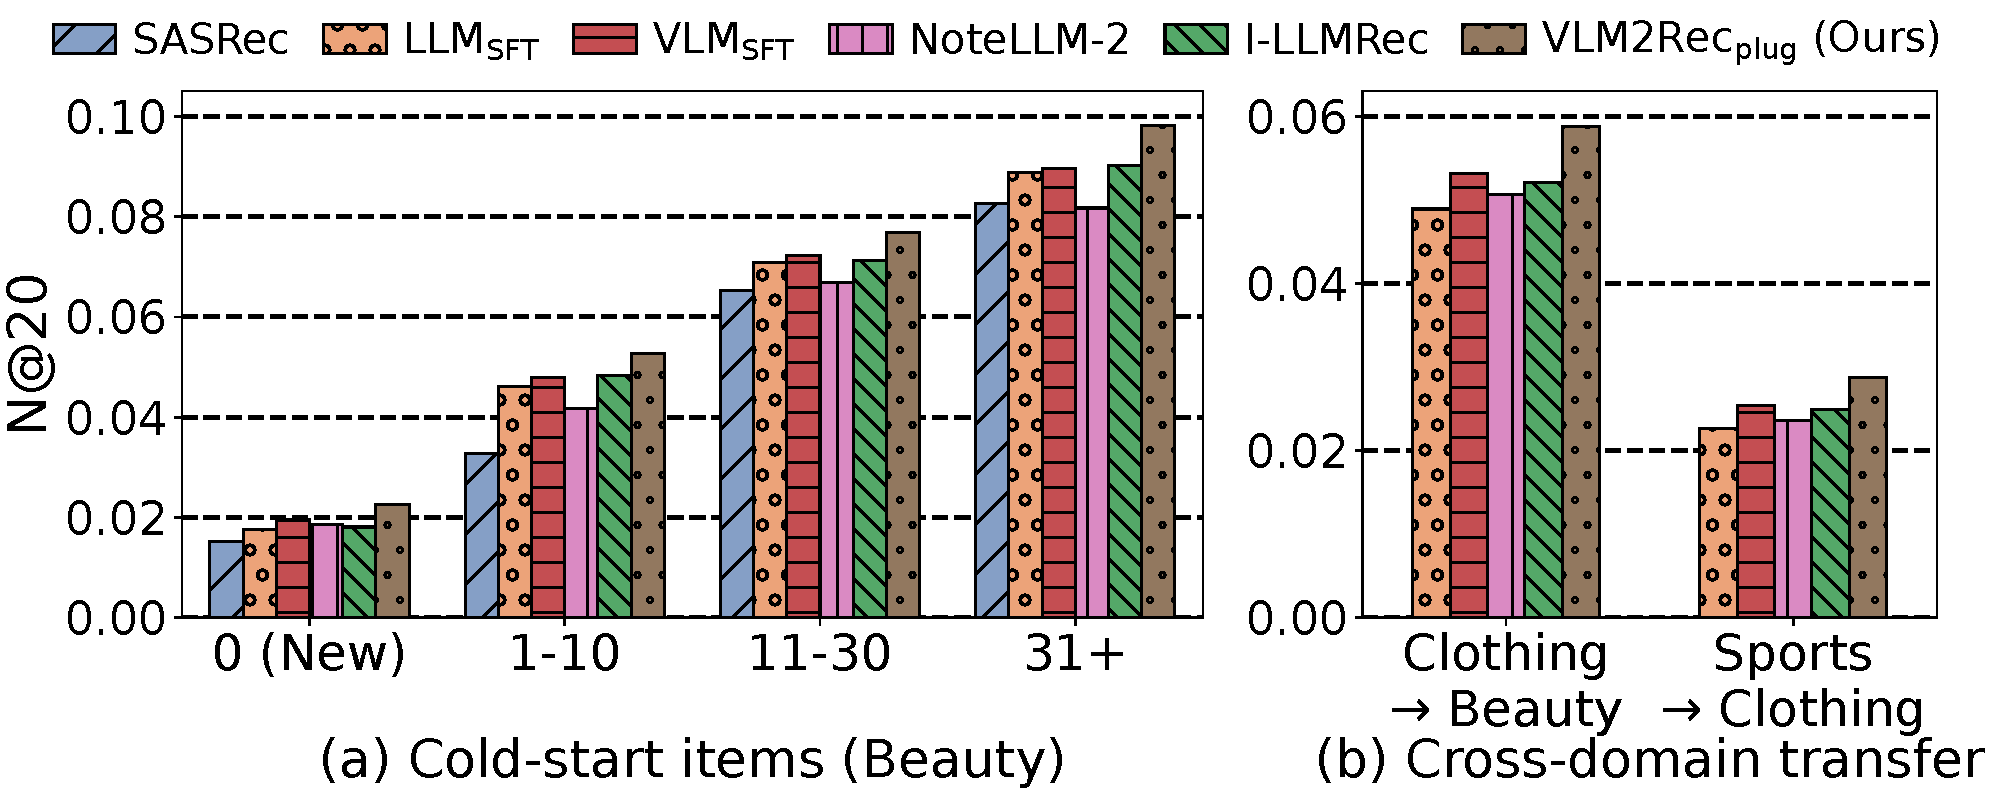
\includegraphics[width=\columnwidth]{figures/cold_cross.pdf}
    % \caption{Performance under scarce CF signals: (a) cold-start items, grouped by the number of training interactions; (b) cross-domain transfer (source $\to$ target).}
    \caption{Scarce CF signals: (a) cold-start items, grouped by training interactions; (b) cross-domain transfer.}
    \label{fig:scarce_cf}
\end{figure}








\subsection{User-level Gap and Rank Recovery Analysis}
\label{sec:user_stratification}

We test whether VLM2Rec reduces the gap consistently across users and whether this reduction relates to its ranking gains (Tab.~\ref{tab:user_stratification}).
\textit{Low} and \textit{High} are the users with the bottom and top 20\% of $\Delta_{u,\mathrm{gap}}$ under $\text{VLM}_{\text{Vanilla}}$, and \textit{Collapse} is the half of \textit{Low} users whose gap grows most under SFT.
VLM2Rec lowers the gap from $\Delta_{u,\mathrm{gap}}^{\text{SFT}}$ to $\Delta_{u,\mathrm{gap}}^{\text{Ours}}$ in every group and for most users (User Red., the share of users whose gap shrinks).
Per-user gap recovery correlates more with the weak modality's rank recovery over $\text{VLM}_{\text{SFT}}$ (Pearson $r$ 0.16--0.46) than with the strong or fused one (at most 0.14), so VLM2Rec's gains are tied more to recovering the weak modality than to refining the fused representation.
To check whether each user-level part of the penalty matters, we test three variants of $w_{u,\text{pen}}$ (Tab.~\ref{tab:penalty_variants}).
First, to test whether a fixed margin explains the gain, we compare a \textit{static} penalty $w_{u,\text{pen}}{=}1+\log 2$, its value without a gap, with removing $w_{u,\text{pen}}$: it recovers little of VLM2Rec's gain, so a fixed margin is not its main source.
Second, to test whether the gap must be measured per user, we compare a \textit{batch-level} penalty from batch-averaged margins with the static one: it helps on MovieLens (+5.9\%), where most users are vision-weak, but barely on Clothing (+1.4\%), where text- and vision-weak users nearly split and their gaps largely cancel in the batch average, so the gap must be measured per user.
Third, to test whether the weak modality must be identified per user, we compare a \textit{modality-fixed} penalty that fixes vision as weak with VLM2Rec: it lowers N@20 by 1.9\% on Clothing, where 46\% of users are text-weak, and by 1.3\% on MovieLens, where 27\% are (Tab.~\ref{tab:user_anchor_split}), so per-user identification is needed (case study in App.~\ref{app:case_study}).



\begin{table}[!t]
    \centering
    \caption{Penalty variants of $\mathcal{L}_{\text{WPCL}}$ in the VLM2Rec setting.}
    \label{tab:penalty_variants}
    \setlength{\tabcolsep}{9pt}
    \resizebox{\columnwidth}{!}{
    \renewcommand{\arraystretch}{0.8}
    \begin{tabular}{lcccc}
    \toprule
    \textbf{Penalty} & \textbf{Gap} & \begin{tabular}[c]{@{}c@{}}\textbf{Weak}\\\textbf{modality}\end{tabular} & \textbf{Clothing} & \textbf{MovieLens} \\
    \midrule
    None & -- & -- & 0.0342 & 0.1131 \\
    Static & -- & -- & 0.0347 & 0.1145 \\
    Batch-level & Batch & Batch & 0.0352 & 0.1212 \\
    Modality-fixed & User & Vision & 0.0363 & 0.1236 \\
    \textbf{User-adaptive} & User & User & \textbf{0.0370} & \textbf{0.1252} \\
    \bottomrule
    \end{tabular}
    }
\end{table}


% Few-shot efficiency is now a figure; the table (tables/few_shot.tex) is no longer input.
\begin{figure}[t]
    \centering
    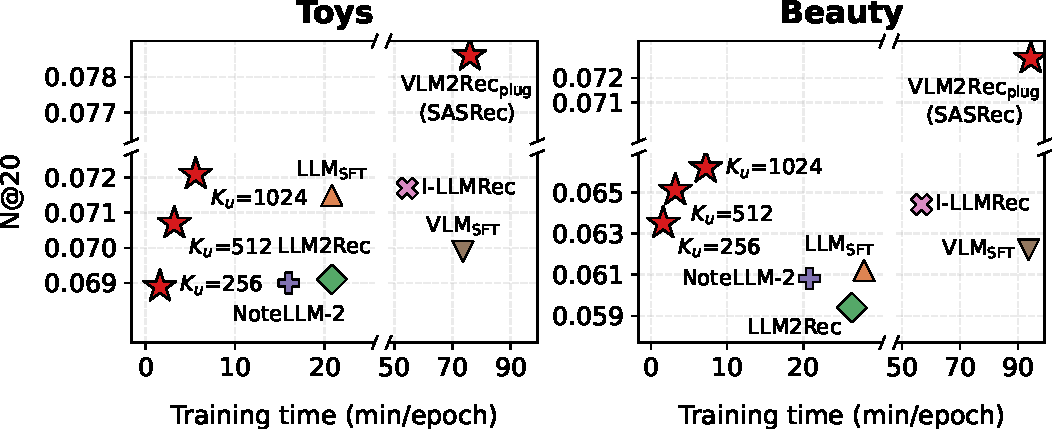
\includegraphics[width=\columnwidth]{figures/few_shot_efficiency.pdf}
    \Description{Two scatter panels, Toys and Beauty, plotting training time per epoch against N@20 with broken axes. VLM2Rec-plug with SASRec trained on all users is the highest point. Its variants trained on 256, 512, and 1024 users take a few minutes per epoch, and the 1024-user variant outperforms every baseline in both panels.}
    \caption{Few-shot efficiency: training time (min/epoch).}
    \label{fig:few_shot}
\end{figure}





\subsection{Generalization under Scarce CF Signals}


We evaluate generalization under scarce CF signals in two settings: \textit{cold-start items} (Fig.~\ref{fig:scarce_cf}a) and \textit{cross-domain transfer} (Fig.~\ref{fig:scarce_cf}b).
\noindent\textbf{Cold-start Analysis}: 
Items are grouped by their training interactions (0, 1--10, 11--30, and 31+), and new items are ranked from their titles and images alone.
Rarer items leave fewer transitions for the backbone to memorize, so ranking them relies more on content semantics; accordingly, $\text{VLM2Rec}_{\text{plug}}$'s relative gain over the ID-only SASRec is largest for items with at most ten training interactions.
\noindent\textbf{Cross-domain Transfer}: The embedder trained on a source domain encodes target-domain items for an SR backbone trained and evaluated on that target; domain shift makes memorized CF signals unreliable.
Here, the multimodal embedders, such as I-LLMRec, transfer better than the text-only $\text{LLM}_{\text{SFT}}$, suggesting that visual preferences carry across domains.
$\text{VLM2Rec}_{\text{plug}}$ achieves the best results in both settings, suggesting that balanced multimodal representations transfer well when CF signals are scarce.


\subsection{Cost and Few-shot Efficiency Study}
\label{sec:few_shot}

Fig.~\ref{fig:few_shot} reports training time (min/epoch) across LLM- and VLM-based methods, and Tab.~\ref{tab:emb_time} reports item embedding generation time.
% $\text{VLM}_{\text{SFT}}$ and $\text{VLM2Rec}_{\text{plug}}$ are more expensive to train than other methods because they process image sequence tokens, but their similar runtimes show that this cost arises from the VLM encoding stage rather than our proposed loss terms. 
$\text{VLM}_{\text{SFT}}$ and $\text{VLM2Rec}_{\text{plug}}$ are more expensive to train than other methods because they process image sequence tokens, but their similar runtimes show that this cost arises from VLM encoding rather than our losses.
% To reduce this cost, we train a few-shot variant trained on $K_u$ random users: at $K_u{=}1024$ (about 5\% of training data), it already exceeds the strongest baseline with much shorter training time.
To reduce this cost, we train a few-shot variant on $K_u$ random users: at $K_u{=}1024$ (about 5\% of training data), it already exceeds the strongest baseline with much shorter training time.
The complexity and hyperparameter analyses confirm that our losses preserve the asymptotic complexity of $\mathcal{L}_{\text{SFT}}$ (Tab.~\ref{tab:complexity_loss}) and that performance is stable across hyperparameters (Fig.~\ref{fig:hyperparameter}).
Performance also grows with VLM size and is similar across families (Fig.~\ref{fig:model_capacity}), so the VLM can be scaled to the compute budget without changing the serving cost of $\text{VLM2Rec}_{\text{plug}}$.

 